\documentclass{article}

% URLs and hyperlinks ---------------------------------------
\usepackage{hyperref}
\hypersetup{
	colorlinks=true,
	linkcolor=blue,
	filecolor=magenta,      
	urlcolor=blue,
}
\usepackage{xurl}
%---------------------------------------------------

\usepackage{graphicx}
\usepackage{rotating}
\usepackage{mathtools}
\usepackage{xepersian}
\settextfont{Yas}

\title{گزارش کار آزمایش دوم:‌\\آشنایی با روش‌های تحلیل مدارهای مقاومتی}
\author{
	گروه: \\
	اریسا احسانی \\
	سید حسین حسینی \\
	مهدی حق‌وردی
}
\date{}
\renewcommand{\arraystretch}{1.4}

\begin{document}
	\maketitle
	\tableofcontents
	\clearpage
	
	\section{تحلیل تقسیم جریان و تقسیم ولتاژ}
		\begin{center}
			
\includegraphics[width=12cm, height=8cm]{./images/1}
		\end{center}
		
		\subsection{توضیحات}
			در این آزمایش، با روابط بین تقسیم جریان و تقسیم ولتاژ‌ در مدارات سری و موازی به صورت عملی آشنا می‌شویم.
			
		\subsection{مقادیر}
		با توجه به مدار بسته شده در نرم‌افزار پروتئوس، ولتاژ نقاط بدین شرح هستند:
		
		\begin{itemize}
			\item \lr{A}: $1.00$ ولت
			\item \lr{B}: $1.00$ ولت 
			\item \lr{C}: $1.00$ ولت
			\item \lr{D}: $0.67$ ولت
			\item \lr{E}: $0.33$ ولت
		\end{itemize}
		که در اینجا، چون \lr{A}، \lr{‌B} و \lr{C} موازی هستند، انتظار می‌رود که مقدار ولتاژ یکسانی داشته باشند. \\
	
		و مقدار جریان‌ها:
		\begin{itemize}
			\item \lr{$I_1$}: $0.10$ میلی‌آمپر
			\item \lr{$I_2$}: $0.03$ میلی‌آمپر
		\end{itemize}
	
		مقادیر عملی بدست آمده در آزمایشگاه:
		\begin{itemize}
			\item \lr{A}: $1.00$ ولت
			\item \lr{B}: $1.00$ ولت 
			\item \lr{C}: $1.00$ ولت
			\item \lr{D}: $0.70$ ولت
			\item \lr{E}: $0.30$ ولت
		\end{itemize}
		
		و مقدار جریان‌ها:
		\begin{itemize}
			\item \lr{$I_1$}: $0.12$ میلی‌آمپر
			\item \lr{$I_2$}: $0.02$ میلی‌آمپر
		\end{itemize}
			با اینکه مقادیر بدست آمده در آزمایشگاه (که چون مقادیر در آزمایشگاه طبیعی هستند و احتمال هرگونه‌ خطایی هست،) با مقادیر نرم‌افزار متفاوت هستند، اما نسبت‌ها و تغییرات بین ولتاژها و جریان‌ها حفظ شده و این یعنی آزمایش به درستی انجام شده و قوانین به صورت تجربی اثبات شده‌اند.
			
	\clearpage
	\section{تحلیل گره}
		\begin{center}
			
\includegraphics[width=12cm, height=8cm]{./images/2}
		\end{center}
		
		\subsection{توضیحات}
			در این مدار و آزمایش قوانین حاکم بر گره‌های موجود در مدار بررسی می‌شود. مواردی که مورد آزمایش و متغیر‌های های موردنظر ولتاژ گره‌ها هستند و ولتاژ گره‌ها نسبت به هم سنجیده می‌شوند.			
			\subsection{مقادیر}
				\begin{center}
					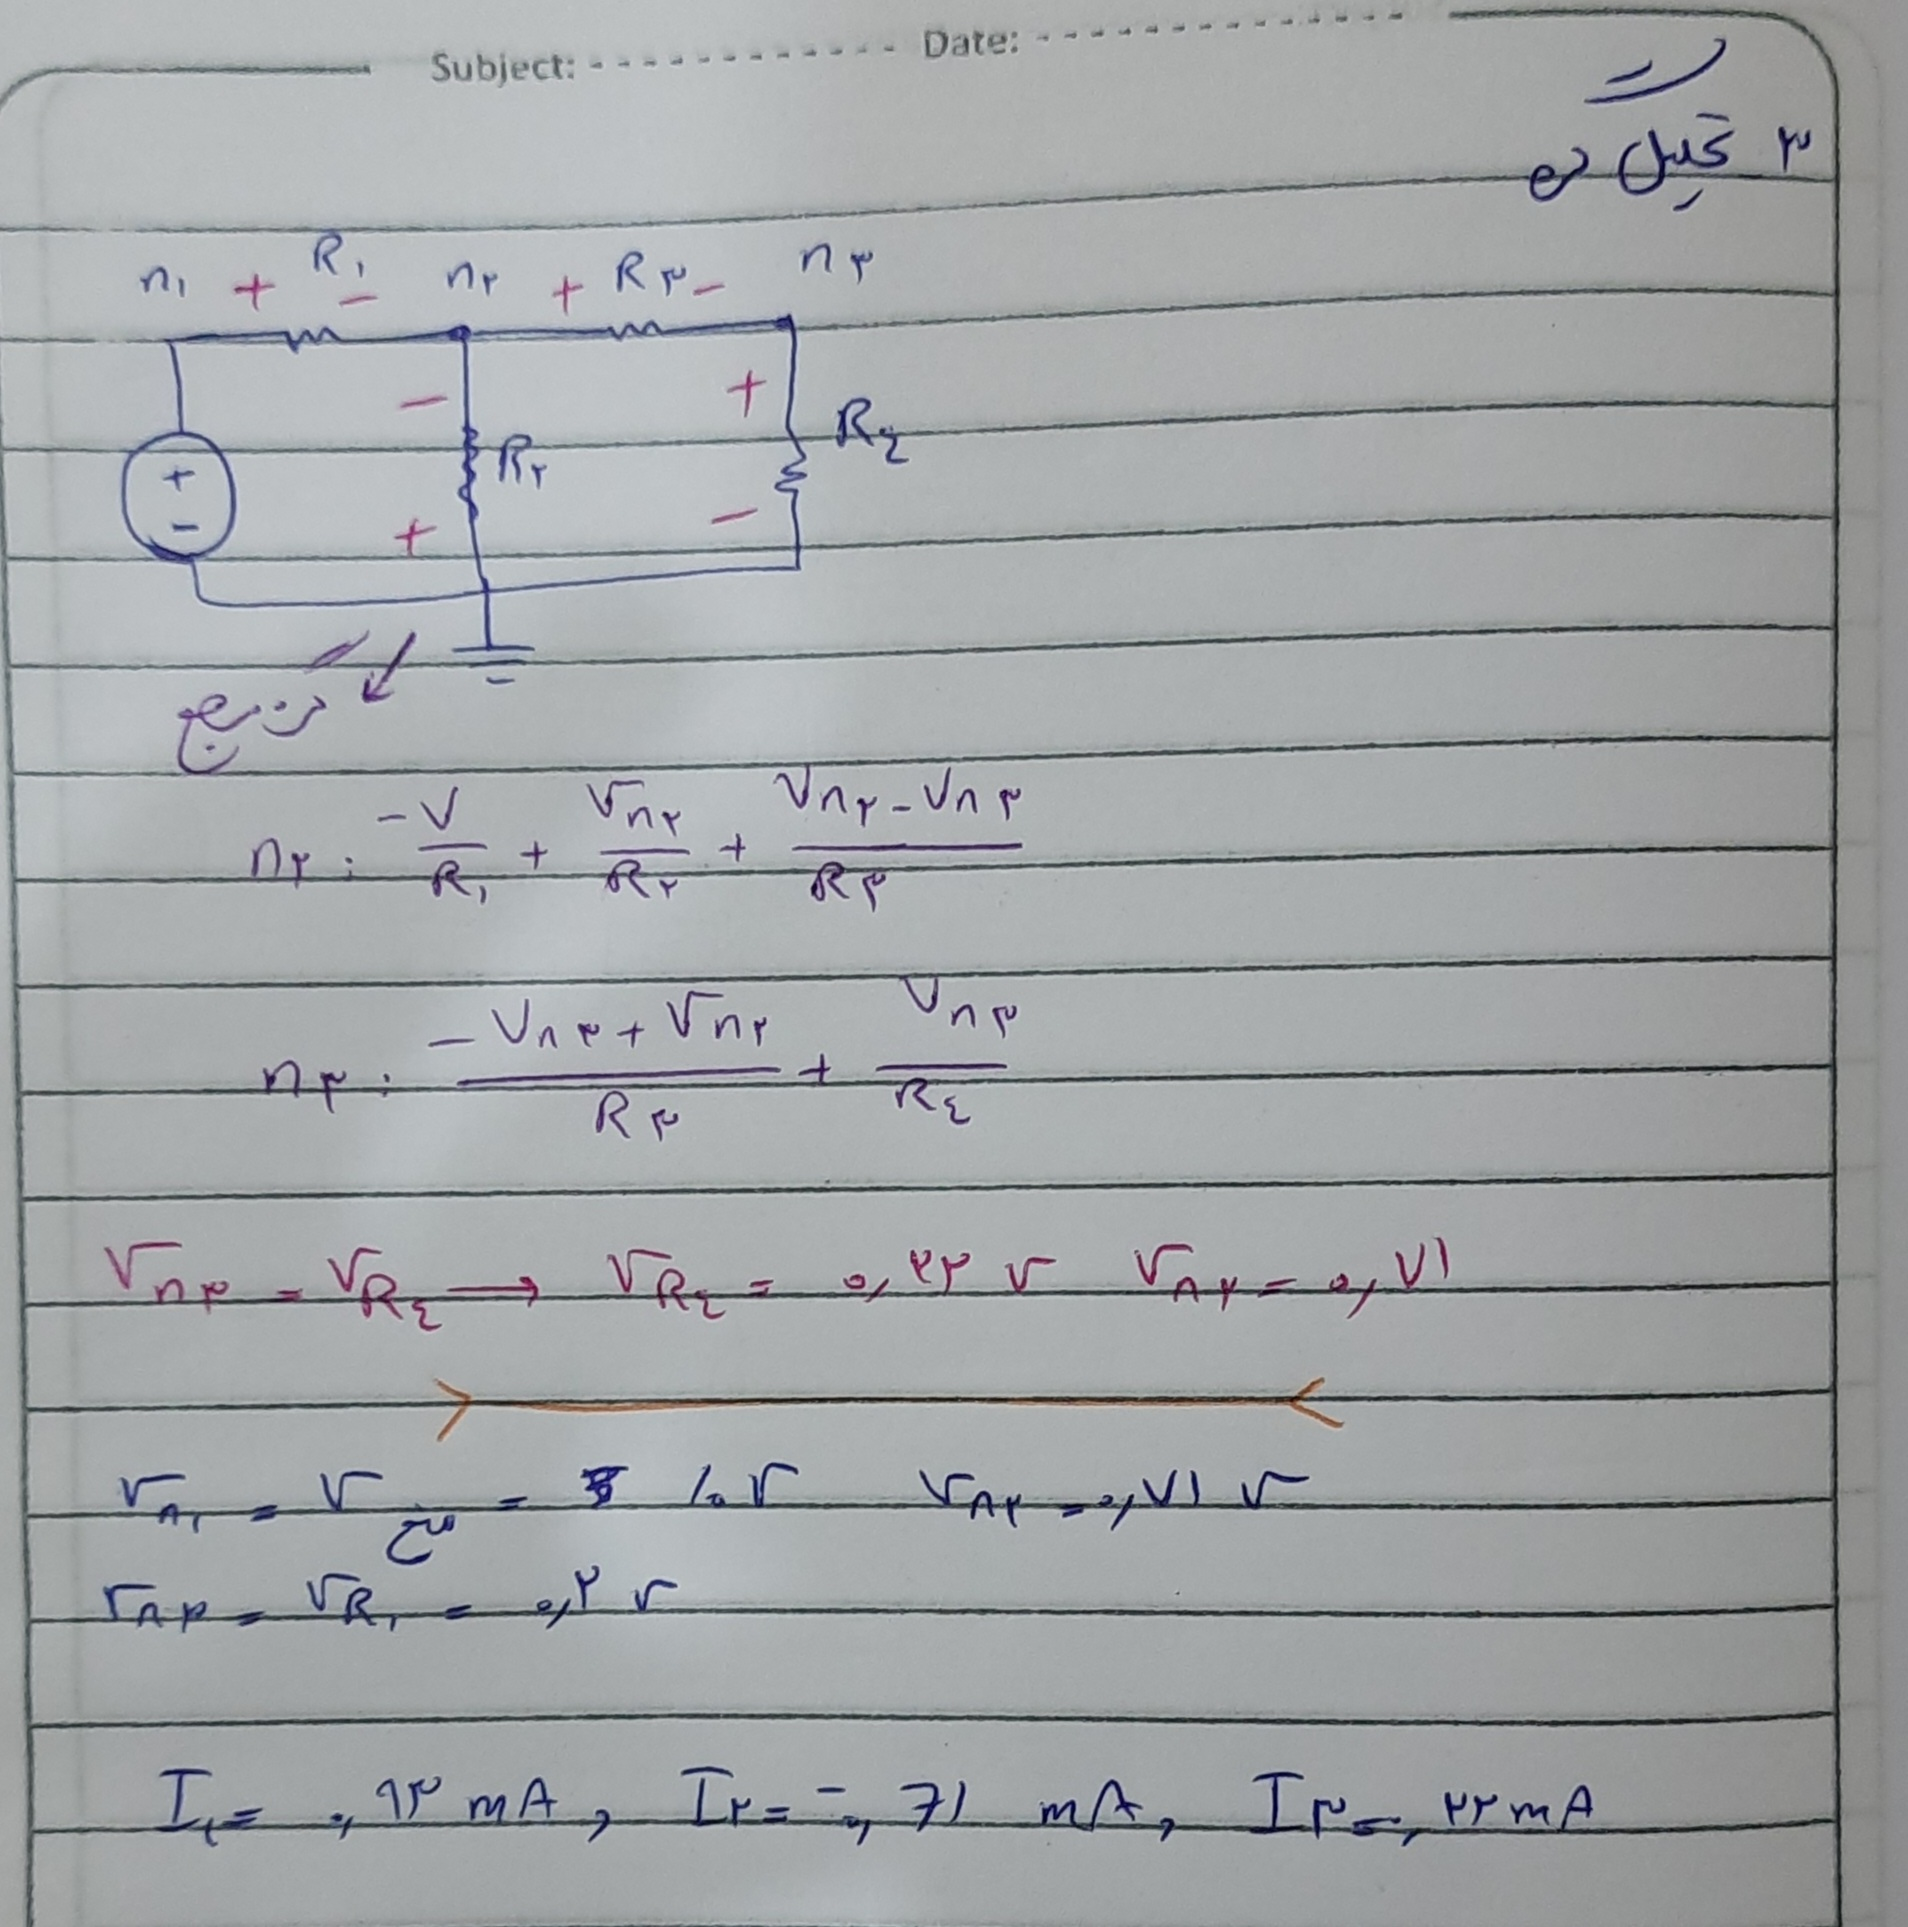
\includegraphics[width=12cm, height=12cm]{./images/2.}
				\end{center}
				\begin{itemize}
					\item 
					اگر ولتاژ دو سر مقاومت $R_7$، $V_2$ باشد، ولتاژ دو سر مقاومت $R_8$ را بدست آورید.
					
					با توجه به مدار بسته شده در نرم‌افزار ولتاژ‌ دو سر مقاومت 
					$V_{R_7} = 0.71 \, V$
					است و مقدار ولتاژ دو سر مقاومت
					$V_{R_8} = 0.22 \, V$
					است.
					
					\item ولتاژ‌ گره‌ها و جریان‌های مسیر‌های مختلف
						\begin{itemize}
							\item \lr{$n_1$} $10$ ولت
							\item \lr{$n_2$} $0.71$ ولت
							\item \lr{$n_3$} $0.22$ ولت
							\item \lr{$I_1$} $0.93$ میلی‌آمپر
							\item \lr{$I_2$} $0.71$ میلی‌آمپر
							\item \lr{$I_3$} $0.22$ میلی‌آمپر
						\end{itemize}
					
					\item توضیحات مقادیر بدست آمده
						\begin{itemize}
							\item ولتاژ‌ها
							
								ولتاژ‌ در این گره‌ها با توجه به نسبت عکس مقاومت‌ها در گره‌ها پخش می‌شود؛ که با توجه به شکل مدار در گره \lr{$n_3$} که مقاومت بیشتری نسبت به گره \lr{$n_2$} دارد، مقدار ولتاژ‌ کمتری هم دارد.
							\item جریان‌ها
								
								با توجه به قوانین موجود بر گره‌‌ها جریان اولیه وقتی به گرهی می‌رسد، در مسیر‌ها پخش می‌شود و در نهایت در موقع برگشت جریان‌ها دوباره با هم جمع می‌شوند که با توجه به مدار می‌توان گفت:‌ $I_1 = I_2 + I_3$ که این با مقادیر بدست آمده هم همخوانی دارد: $0.93 = 0.71 + 0.22$.
								
						\end{itemize}
				\end{itemize}
				
				به دلیل نبود وقت، آزمایش در آزمایشگاه انجام نشد.
				
	\clearpage
	\section{تحلیل مش}
		\begin{center}
			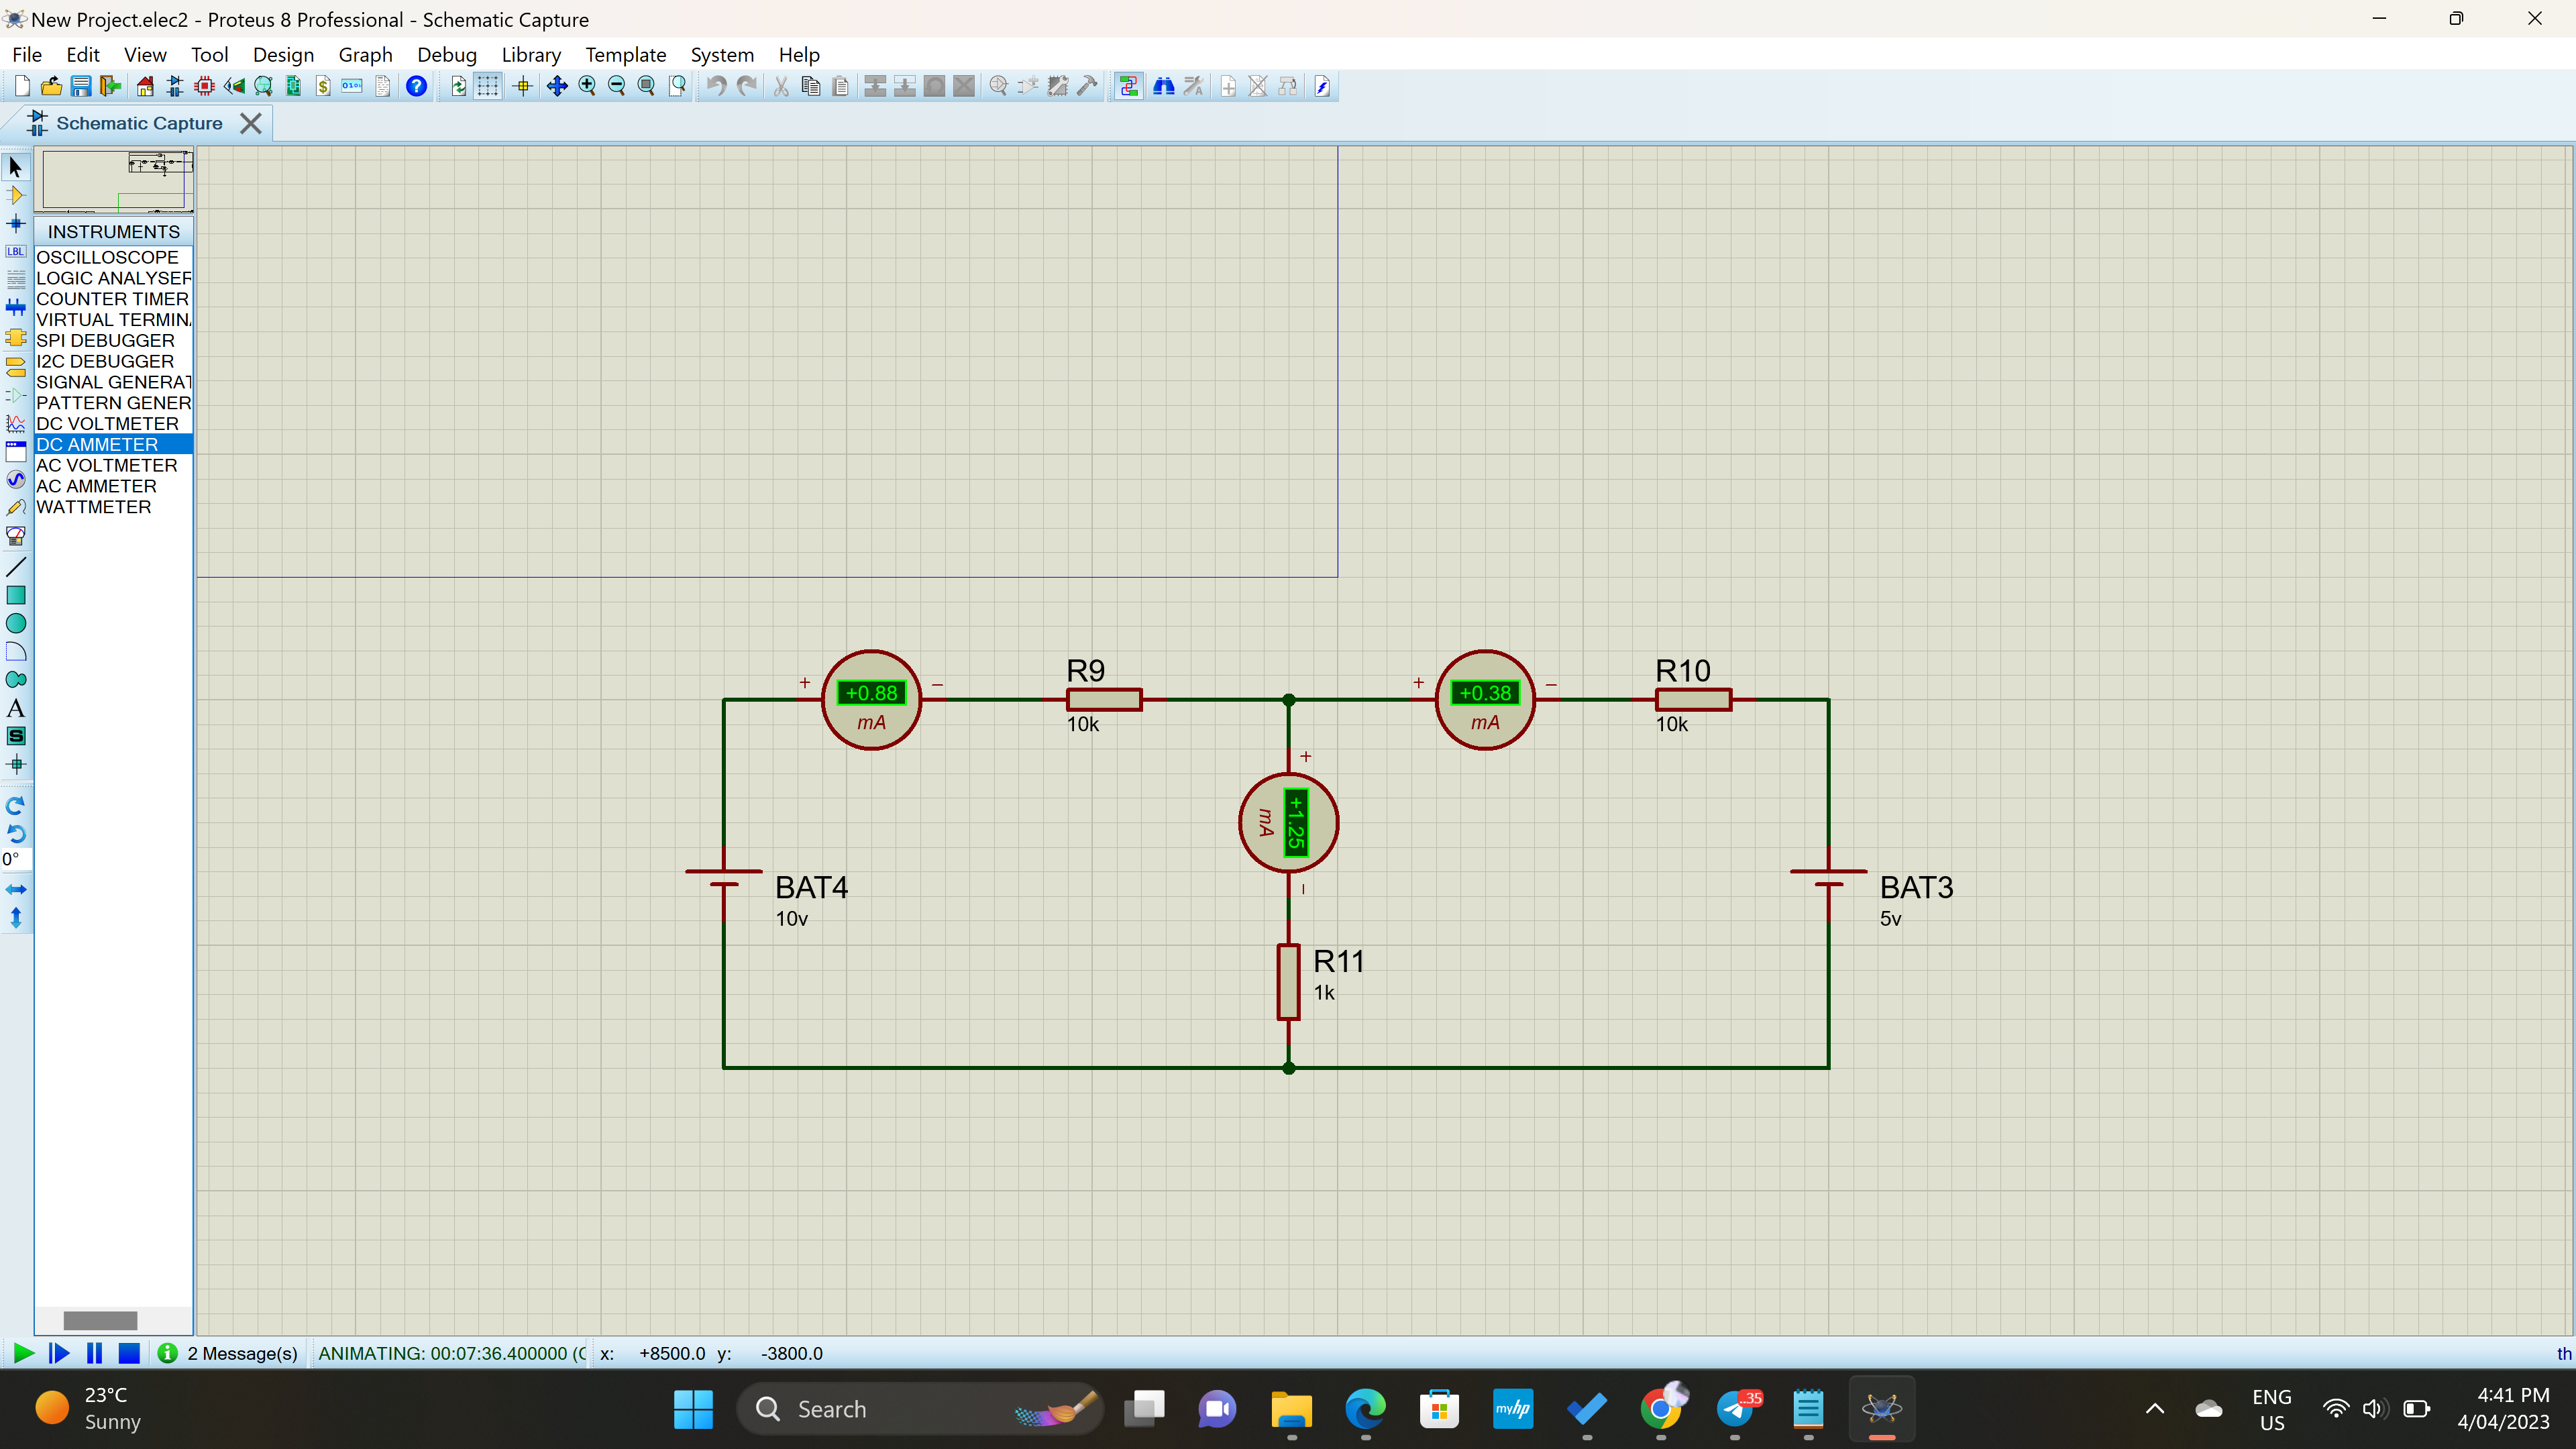
\includegraphics[width=12cm, height=8cm]{./images/3_1}
		\end{center}
		
		\subsection{توضیحات} 
			یکی از روش‌های سریع‌تر و راحت‌تر کردن محاسبات در حل و تحلیل مدار‌ها، استفاده از روش مش با کمک قانون جریان کیرشهف است. به گونه‌ای که برای هر حلقه‌ی مدار، جریان فرضی درنظر می‌گیریم و قانون ولتاژ کیرشهف را برای حلقه می‌نویسیم.
			
			پلاریته‌ی اجزای مدار در تصویر مشخص شده است.
		
		\subsection{مقادیر}	
		\begin{center}
			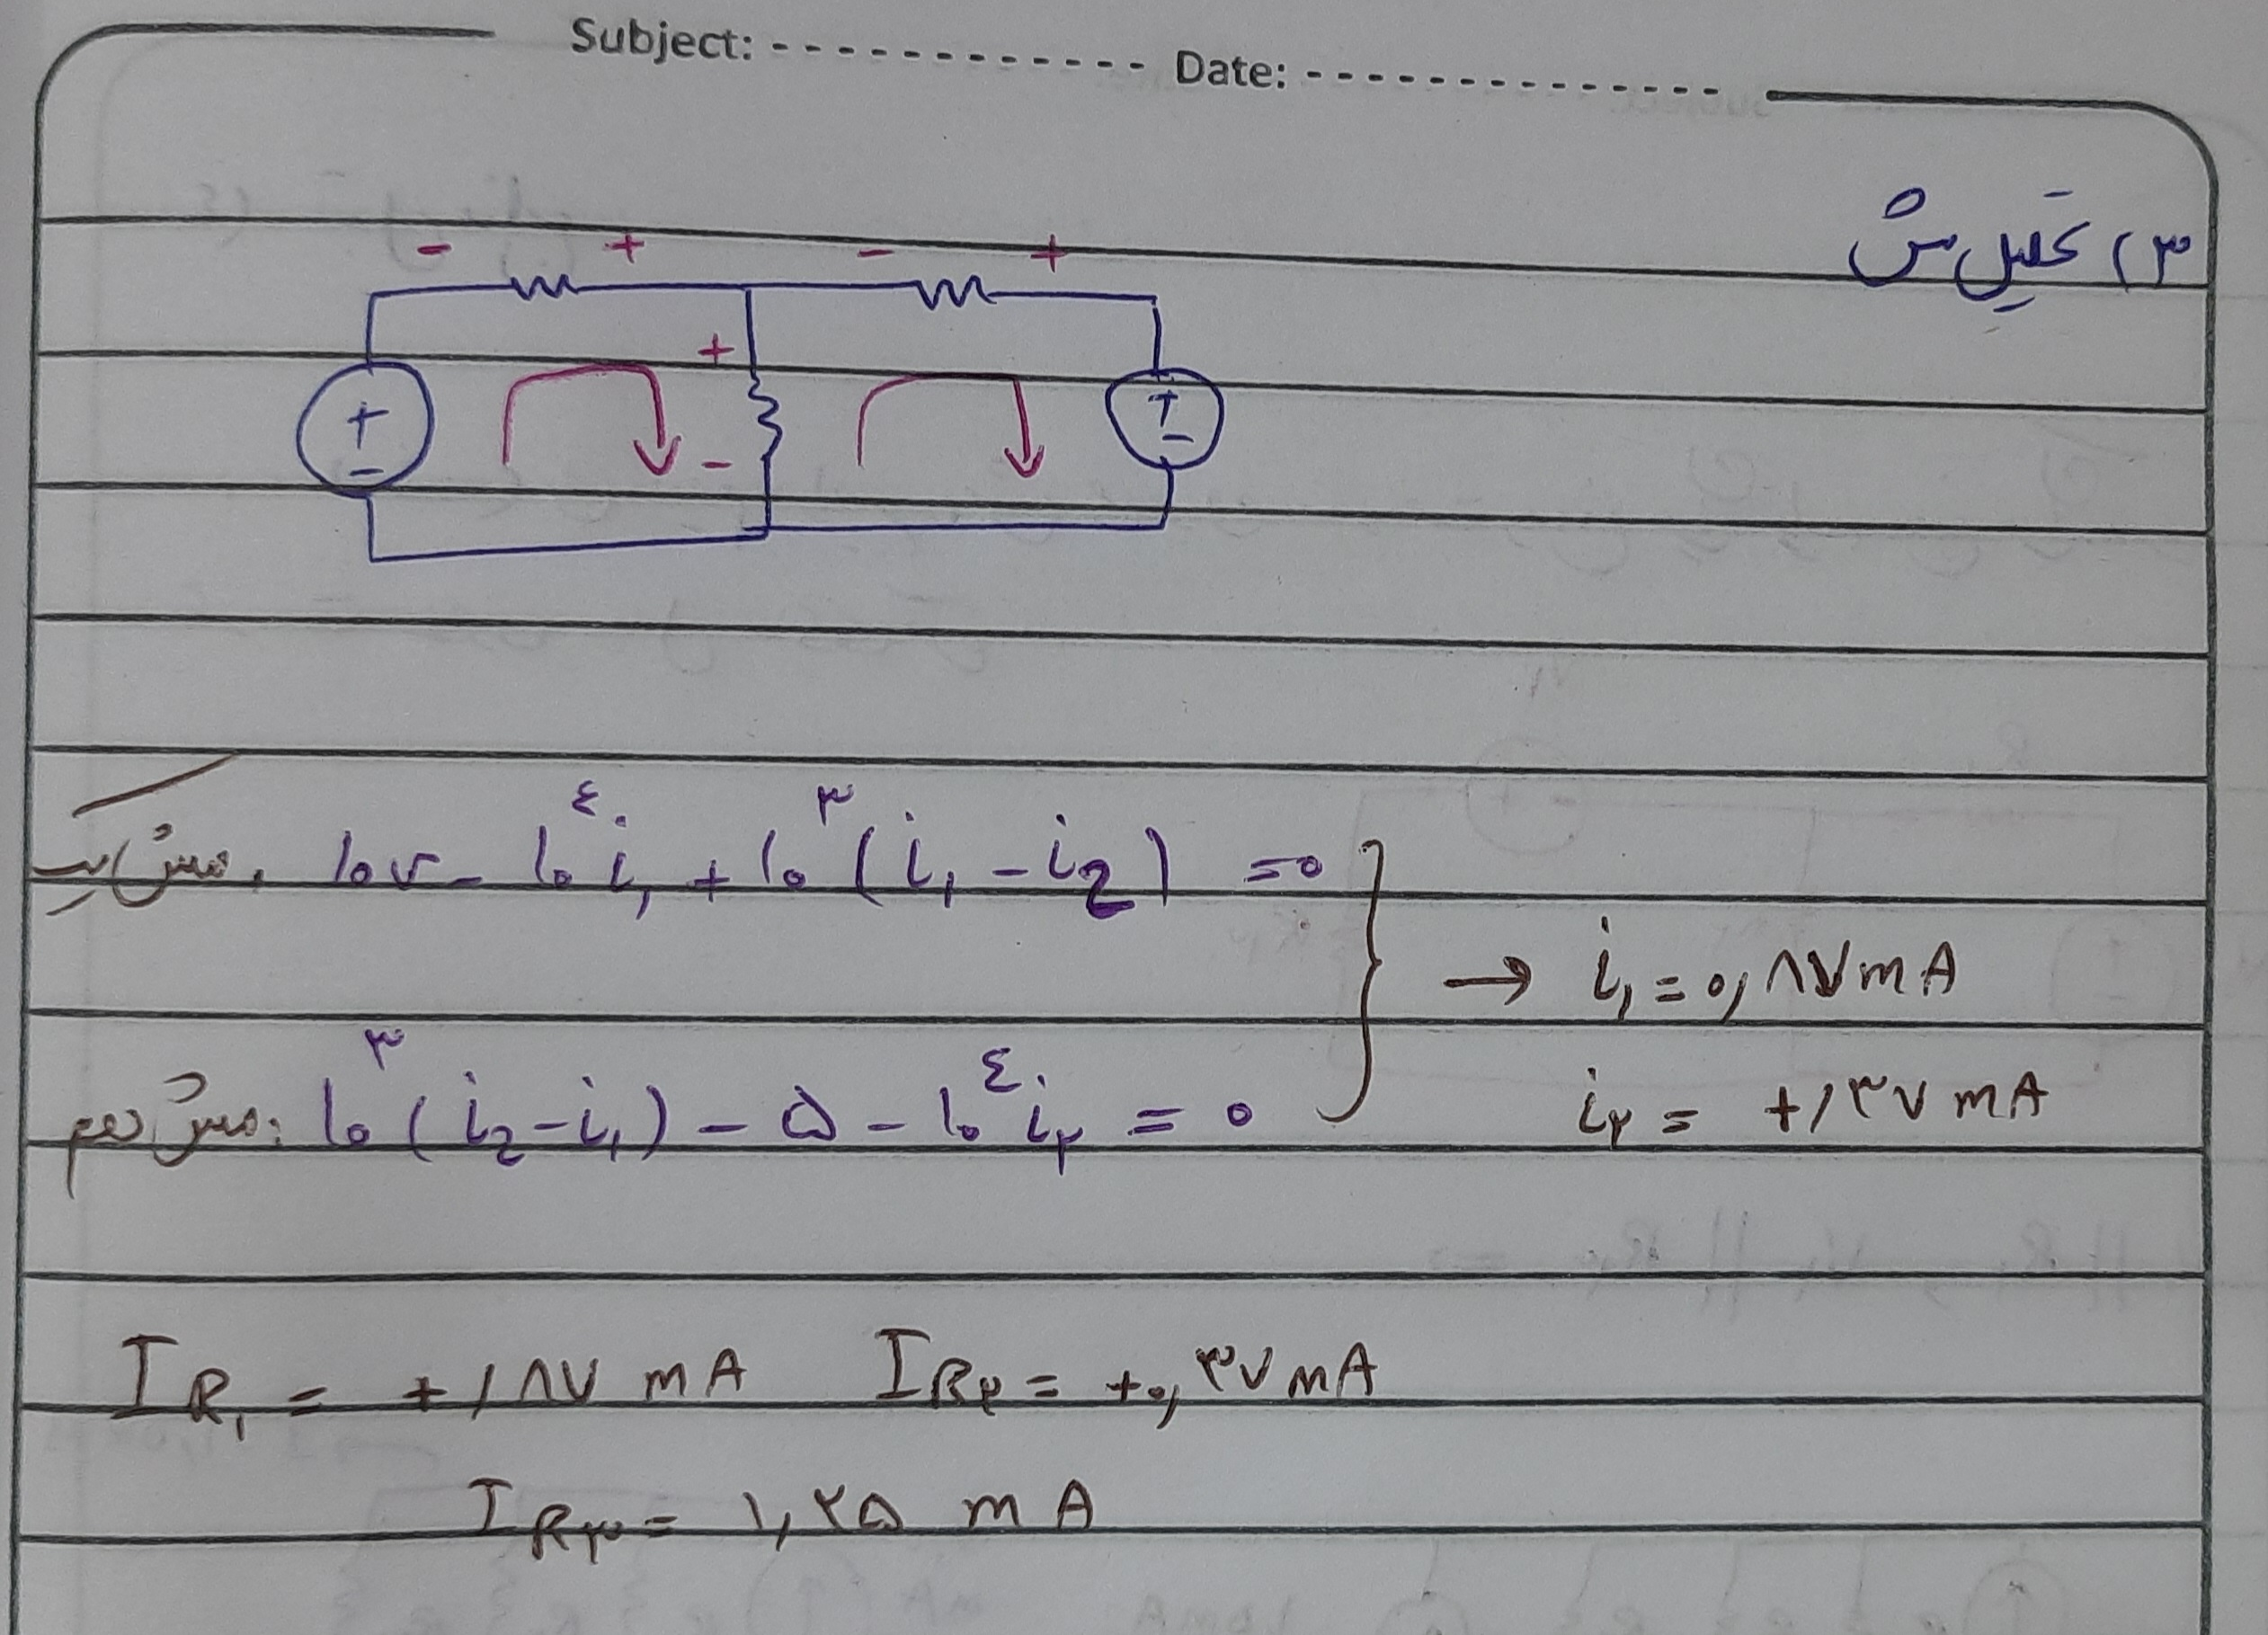
\includegraphics[width=12cm, height=10cm]{./images/3.}
		\end{center}
			مقادیر جریان‌های عبوری
			\begin{itemize}
				\item \lr{$R_9$}: $0.88$ میلی‌آمپر
				\item \lr{$R_{10}$}: $0.38$ میلی‌آمپر
				\item \lr{$R_{11}$}: $1.25$ میلی‌آمپر
			\end{itemize}
		به دلیل نبود وقت، آزمایش در آزمایشگاه انجام نشد.
		
		در یک بند توضیح بدهید که از هر یک روش‌های بالا چه موقع برای تحلیل مدار استفاده می‌شود؟
		در قسمت توضیحات هر روش گفته شد که از روش تحلیل گره متغیر‌ها و خواسته‌ها ما مقدار ولتاژ است و در روش تحلیل مش، متغیر مسئله میزان جریان عبوری است. پس در مسئله‌‌هامان با توجه به متغیر خواسته شده از روش مناسب استفاده می‌شود.
	\clearpage
	\section{تبدیل منابع}
		\begin{center}
			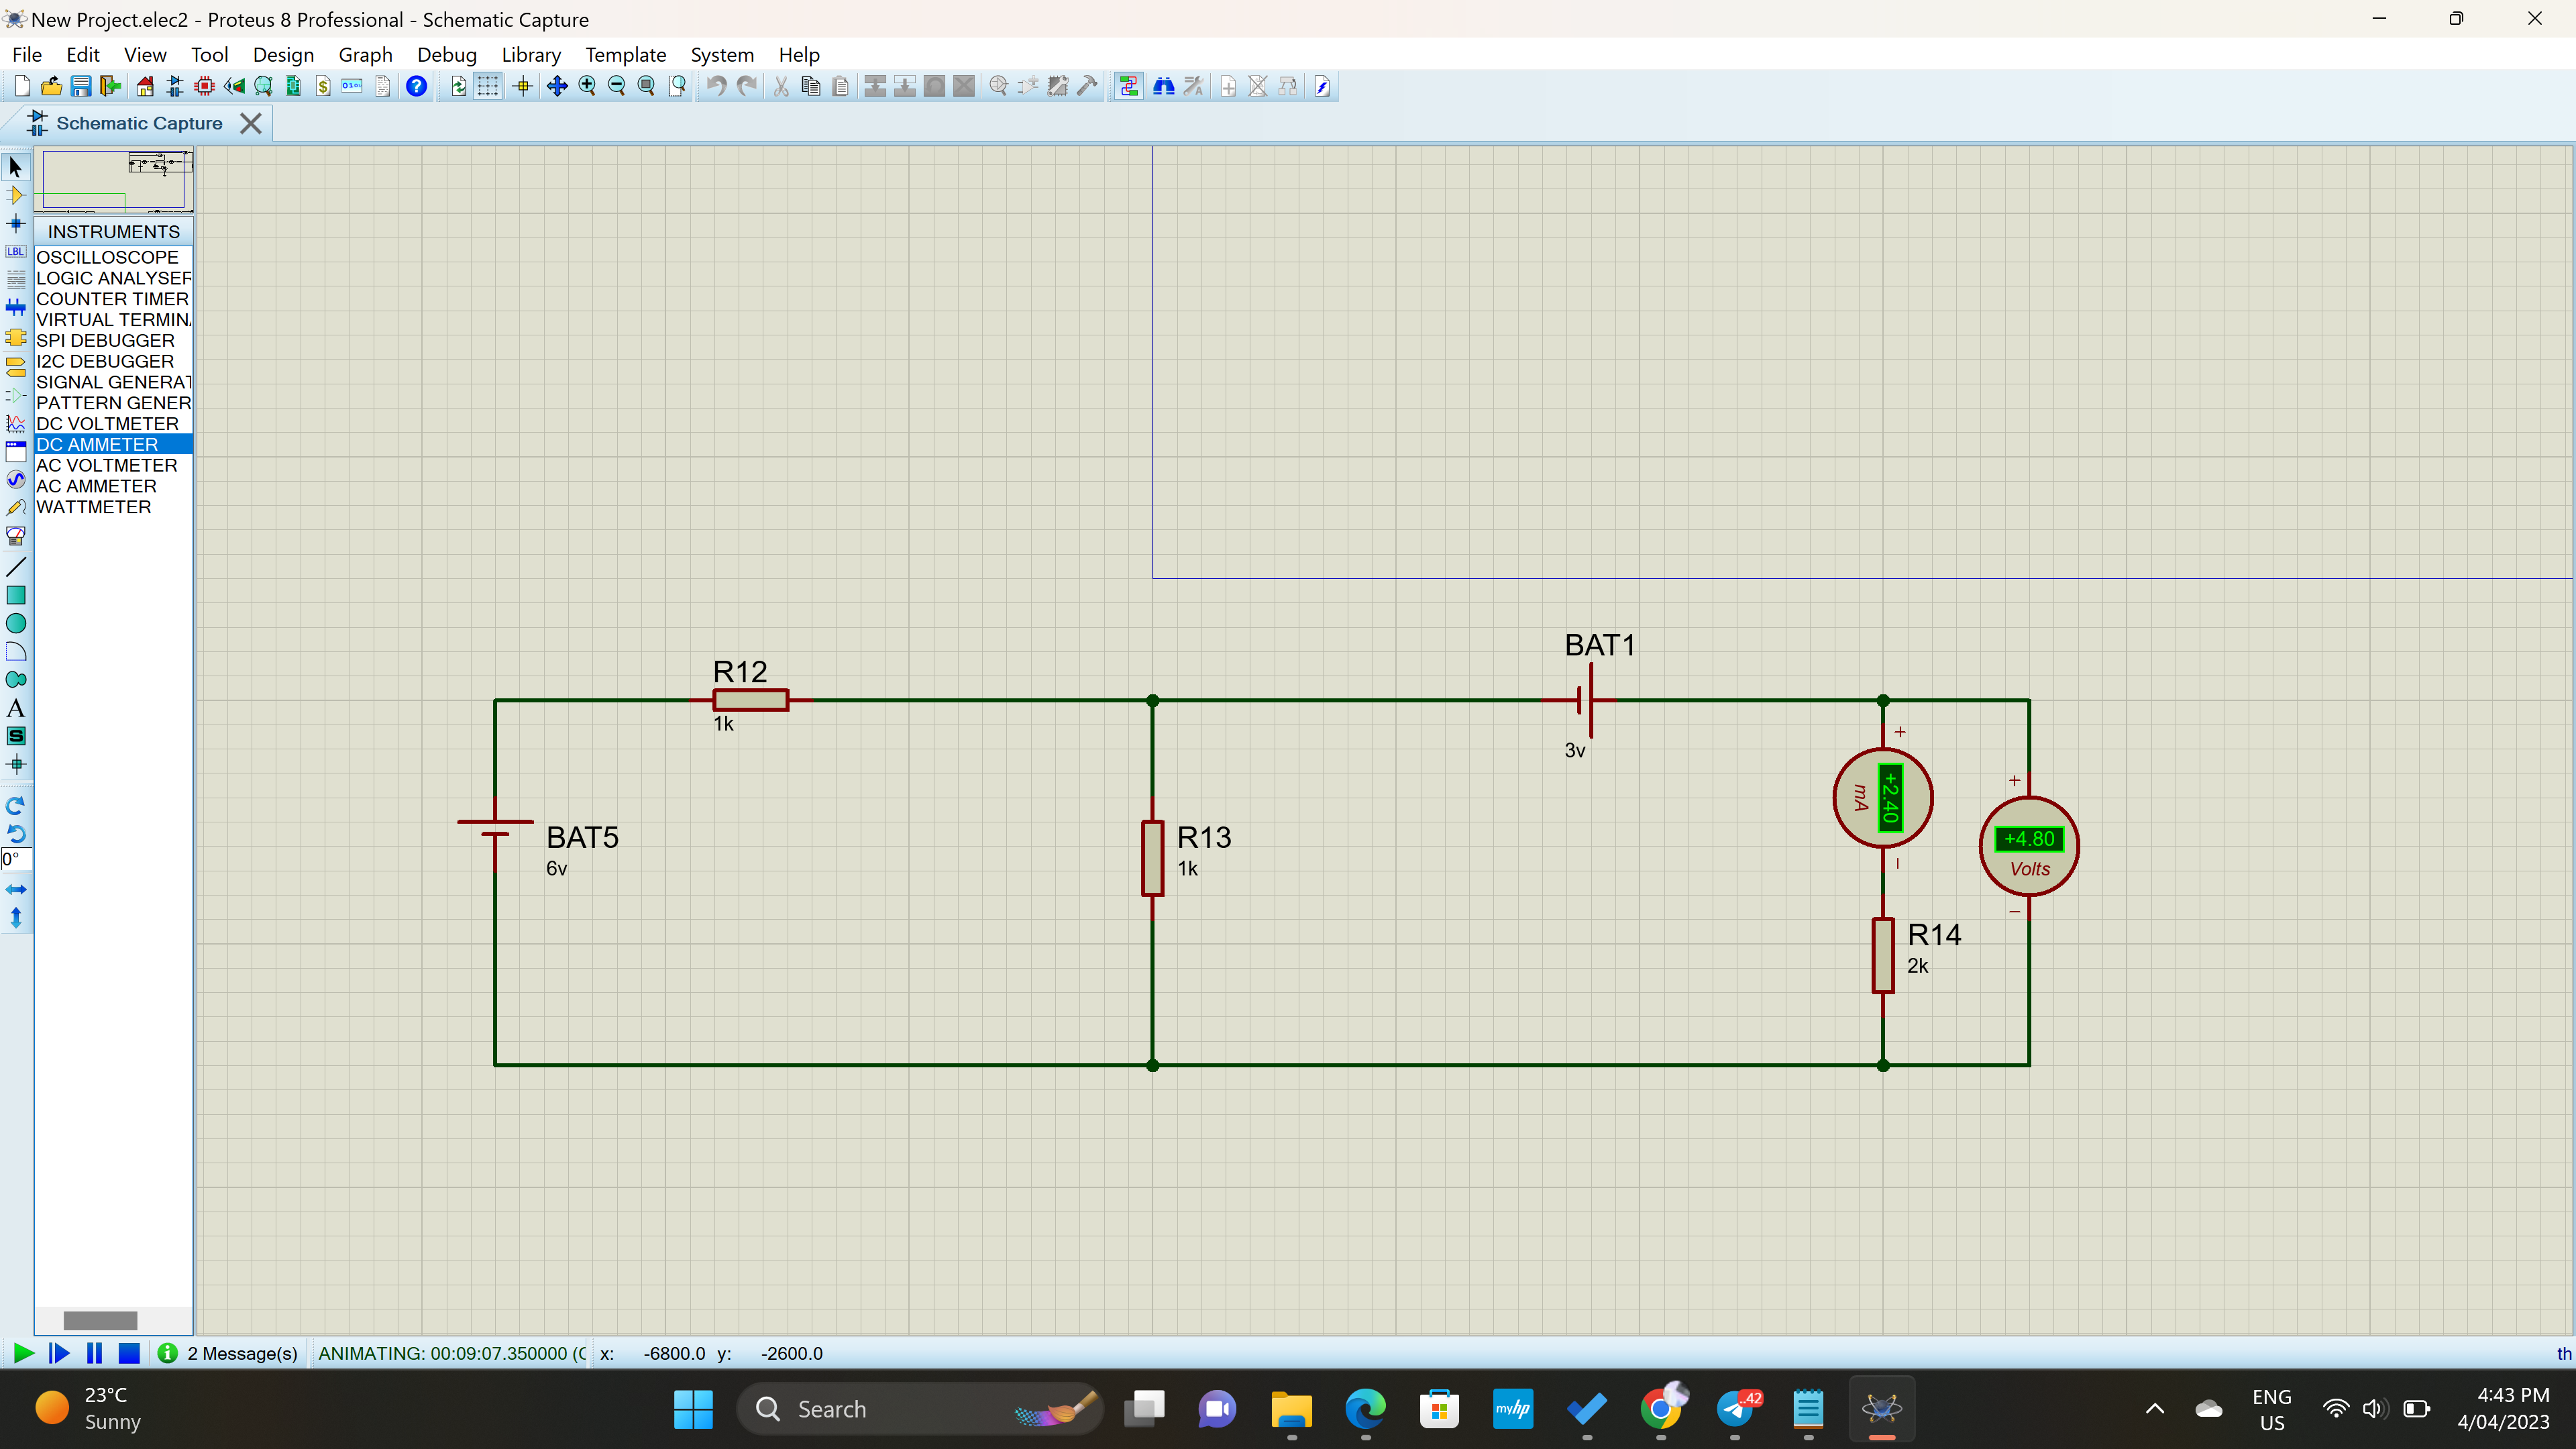
\includegraphics[width=12cm, height=8cm]{./images/3_2}
		\end{center}
		
		\subsection{توضیحات}
			در مدار‌ها، بسته به طرز قرار گرفتن المان‌ها، گاهی حضور منبع جریان در حل معادلات بسیار موثرتر از منبع ولتاژ است و گاهی برعکس. این روش بیان می‌دارد که منبع ولتاژ و یک مقاومت سری با منبع جریان و یک مقاومت موازی برابر هستند، و می‌توان در محاسبات به جای هم استفاده‌شان کرد.
			
			پلاریته‌ی اجزای مدار در تصویر مشخص شده است.
		\subsection{مقادیر}
			\begin{center}
				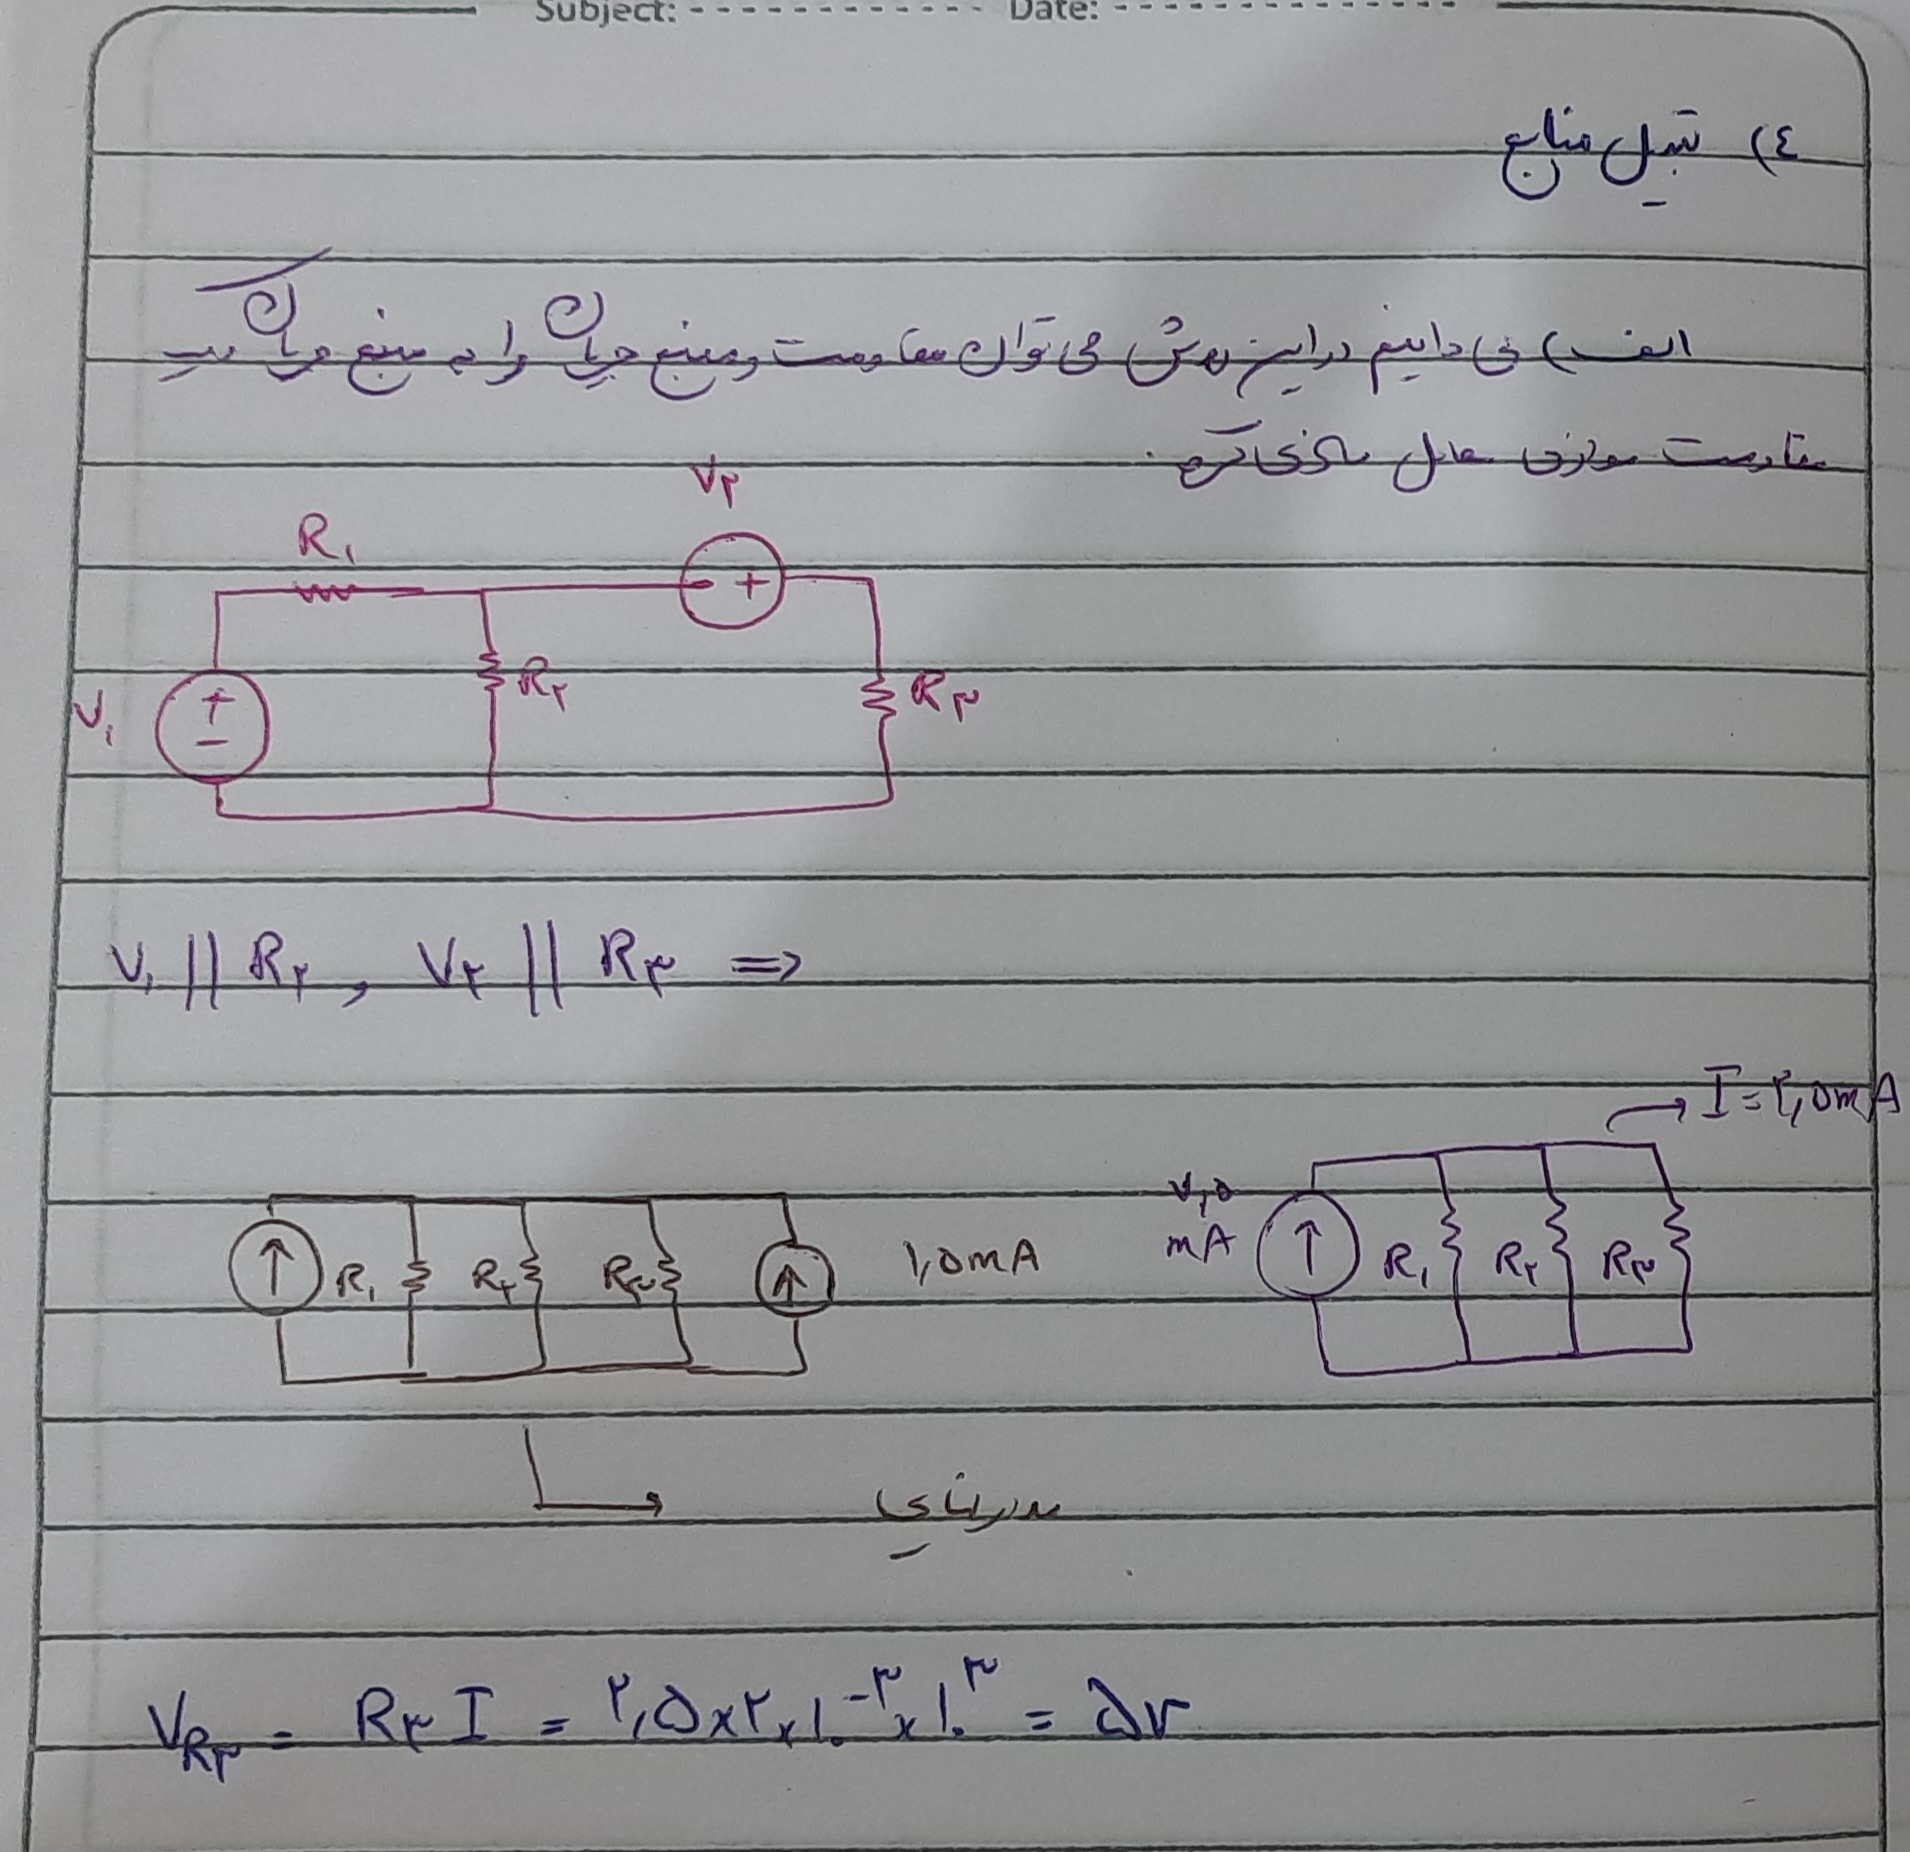
\includegraphics[width=12cm, height=10cm]{./images/4}
			\end{center}
		
			ث) با تغییر سطح مقاومت‌‌ها میزان خطا در محاسبات نیز تغییر می‌کند.
	\clearpage
	\section{قانون جمع آثار}
		\begin{center}
			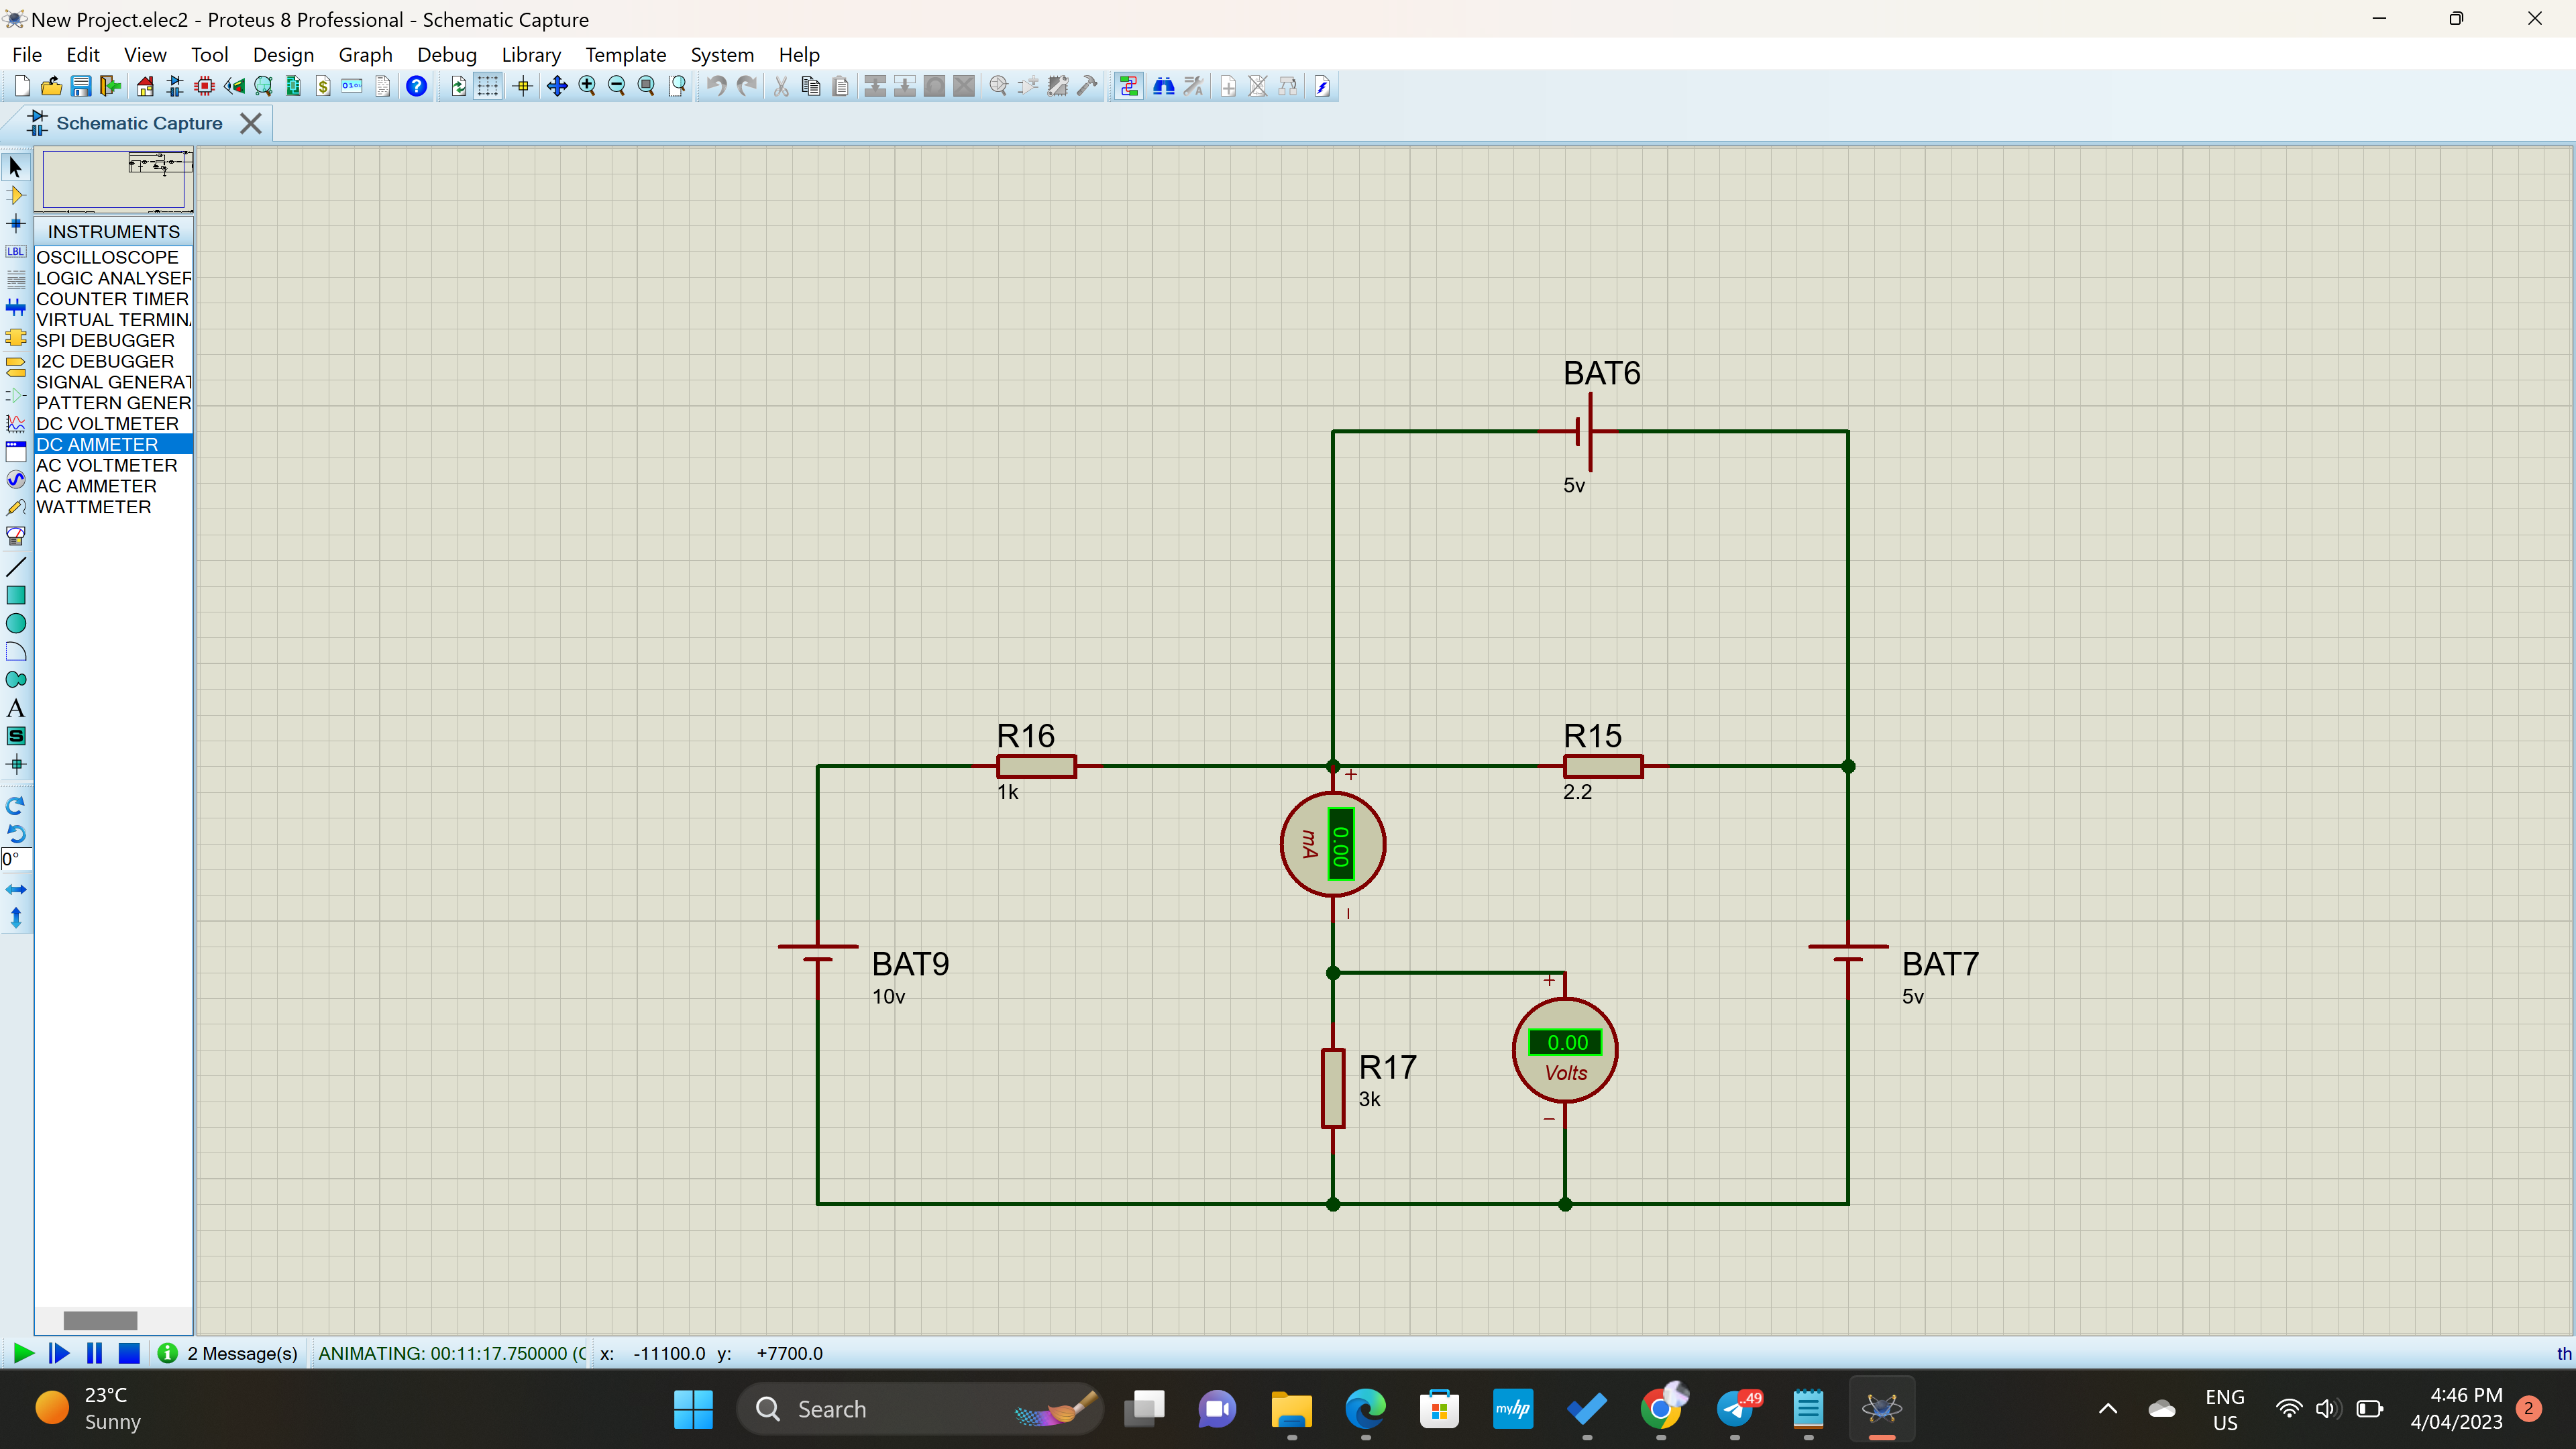
\includegraphics[width=12cm, height=8cm]{./images/3_3}
		\end{center}
		
		\subsection{توضیحات}
			این روش، برای مدار‌هایی که شامل چند منبع مستقل هستند استفاده می‌شود. این قضیه بیان می‌دارد که مقدار مجهول مدار را می‌توان با جمع اثرات ناشی از هر منبع مستقل هنگامی که به تنهایی کار می‌کند محاسبه کرد.
			
			پلاریته‌های اجزای مدار در عکس مشخص شده است.
		\subsection{مقادیر}
			\begin{itemize}
				\item 
				بعد از اتصال کوتاه منابع $V_2$ و $V_3$ مقاومت $R_{17}$ هم اتصال کوتاه می‌شود:
				$V_{R_{17}} = 0 \, V$
				
				\item 
				حذف همه‌ی منابع به جز $V_3$:
				$V_{R_{17}} = 1.6 \times 3 = 4.8 \, V$
				
				\item 
				حذف همه‌ی منابع به جز $V_2$:
				$V_{R_{17}} = 1.4 V \Rightarrow V_{t R_{17}} = 6.2 \, V$
				
				که مقدار بدست آمده در شبیه‌ساز $1.9 \times 3 = 5.7 \, V$ است که مقدار کمی تفاوت دارد.
			\end{itemize}
		
			قسمت ذ: بله با توجه به محاسبات و نتایج نرم‌افزار، بله این روش، روش خوبی برای محاسبات است.
\end{document}